\documentclass[11pt,letterpaper,twoside]{article}
\usepackage[english]{babel}
\usepackage{amssymb,amsmath}
\usepackage{fancyhdr}
\usepackage{graphicx}

 \oddsidemargin  0in \evensidemargin 0in
 \topmargin   -0.25in \headheight 0.25in \headsep 0.25in
 \textwidth   6.5in \textheight 8.75in \marginparsep 0pt \marginparwidth 0pt
 \parskip 1ex  \parindent 0ex \footskip 20pt

\newfont{\bssten}{cmssbx10}
\newfont{\bssnine}{cmssbx10 scaled 900}

%%%%%%%%%%%%%%%%%%%%%%%
\newcommand{\whatizit}{Lecture 2: Data Basics}
%%%%%%%%%%%%%%%%%%%%%%%


\pagestyle{fancy}  
\fancyhead{\bssnine STOR 155,  \whatizit}
\fancyhead[RE]{} \fancyhead[LO]{}
\fancyhead[LE]{\bssnine \thepage} \fancyhead[RO]{\bssnine \thepage}
\lfoot{} \cfoot{} \rfoot{}   


\newcommand{\var}{\mathrm{Var}}



\begin{document}



\thispagestyle{empty} \vspace*{-0.75in}

{\bssten STOR 155: Introduction to Data Models and Inference \hfill May 15, 2024 \\
Prof. Will Lassiter  \hfill Page 1 of \pageref{totalpag}}
\vspace{10pt}
\begin{center} {{\Large \bf \whatizit}} \end{center}

{\bf Data Sets: Vocabulary} \vspace{6pt}

Open the spreadsheet {\tt loan50.xlsx}

Each row of the sheet corresponds to... \vspace{50pt}

Each column of the sheet corresponds to... \vspace{50pt}

Two types of variables:

\begin{itemize}

\item {\bf Numerical} \vspace{100pt}

\item {\bf Categorical} \vspace{100pt}

\end{itemize}

Classifying variables in the {\tt loan50} dataset: \vspace{100pt}

\newpage

{\bf Relationships between Variables} \vspace{6pt}

Open the spreadsheet {\tt county.xlsx}

\begin{center}
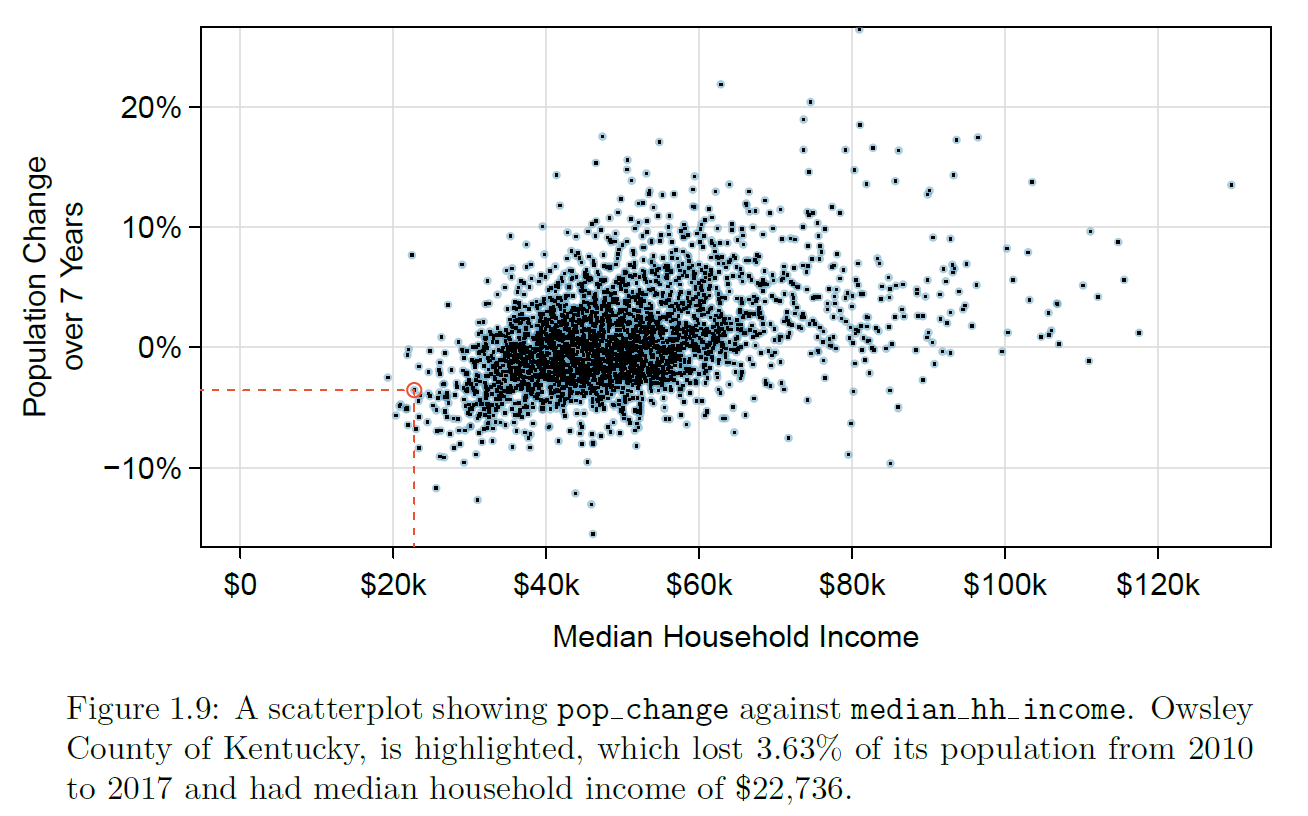
\includegraphics[scale=0.7]{images/scatter1.png}
\end{center}
\vspace{-10pt}
Comments on relationship between median household income and population change? \vspace{80pt}

\begin{center}
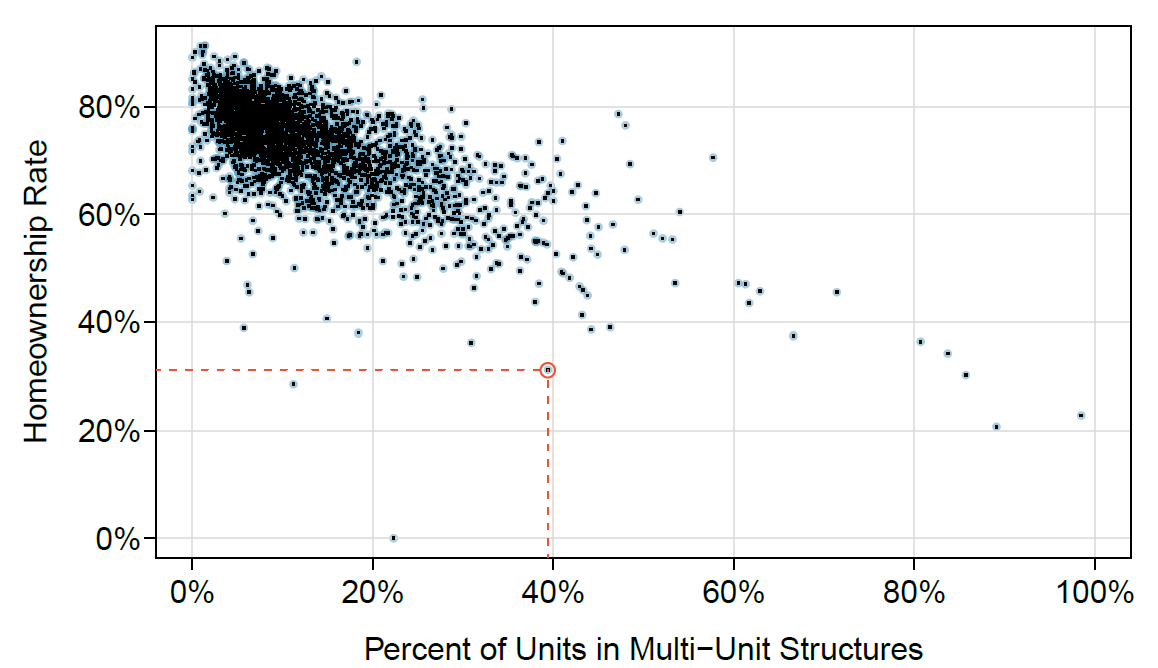
\includegraphics[scale=0.7]{images/scatter2.png}
\end{center}
\vspace{-10pt}
Comments on relationship between these two variables?

\newpage

When examining the relationship between two variables, it is important to establish... \vspace{200pt}

More examples:

\begin{itemize}
\item X: number of beers consumed \\
	Y: blood alcohol content (BAC)
\item X: type of treatment given (drug or placebo) \\
	Y: outcome (cured or not)
\item X: height of an individual \\
	Y: weight of an individual
\item X: SAT verbal score \\
	Y: SAT math score \vspace{40pt}
\end{itemize}

When two variables exhibit some form of relationship, we say they are... \vspace{60pt}

When two variables do not appear to be related, we say they are...

\newpage

{\bf What we consider when describing the relationship between two variables:}
\begin{enumerate}
\item 

\item \vspace{80pt}

\item \vspace{80pt}
\end{enumerate}

\vspace{80pt}

\begin{center}
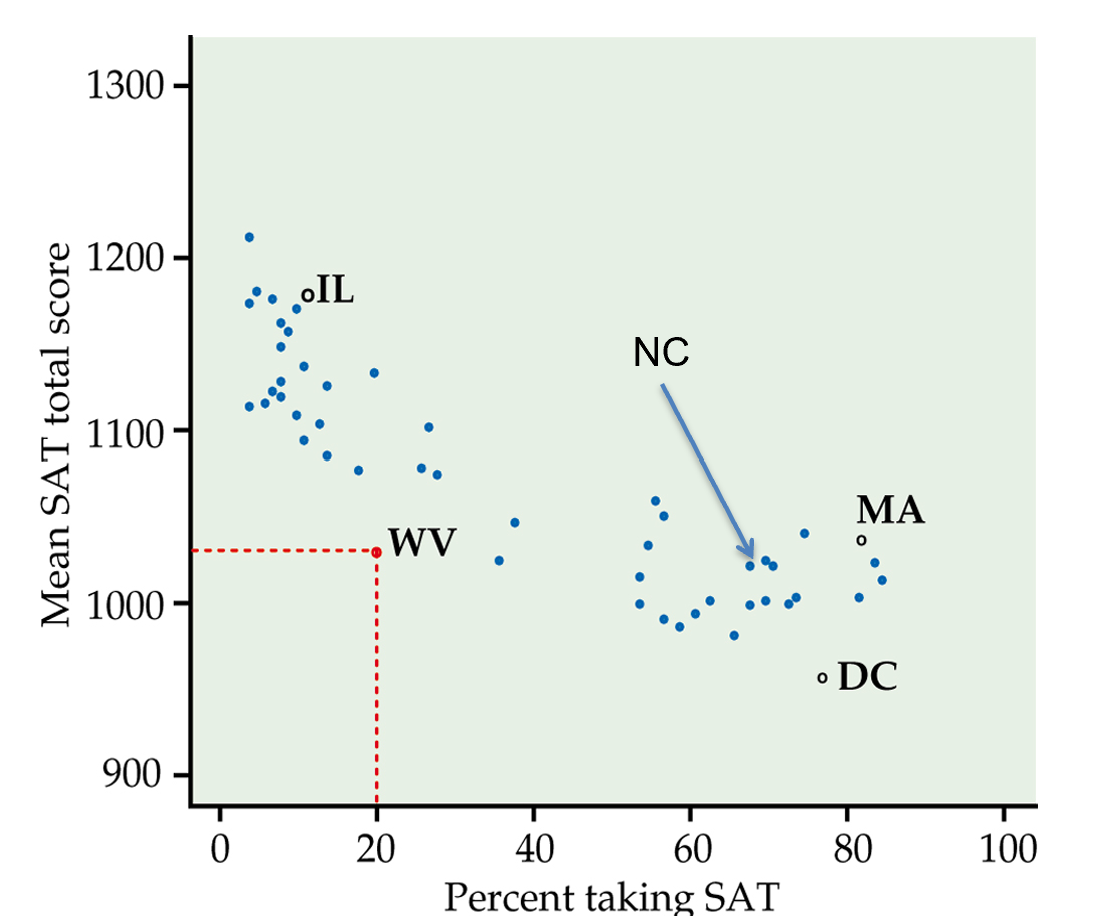
\includegraphics[scale=0.85]{images/scatter3.png}
\end{center}

\newpage

Practice with describing direction and strength:

\begin{center}
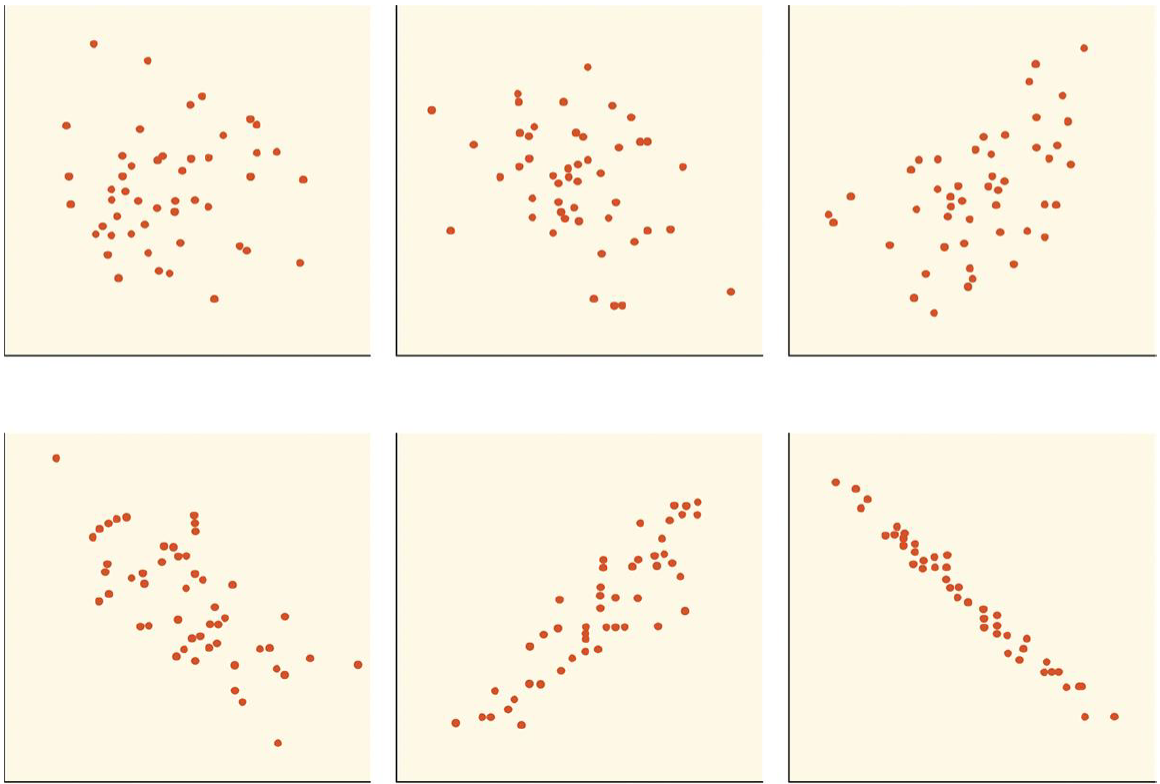
\includegraphics[scale=0.5]{images/scatters.png}
\end{center}
\vspace{10pt}
Practice with describing form:

\begin{center}
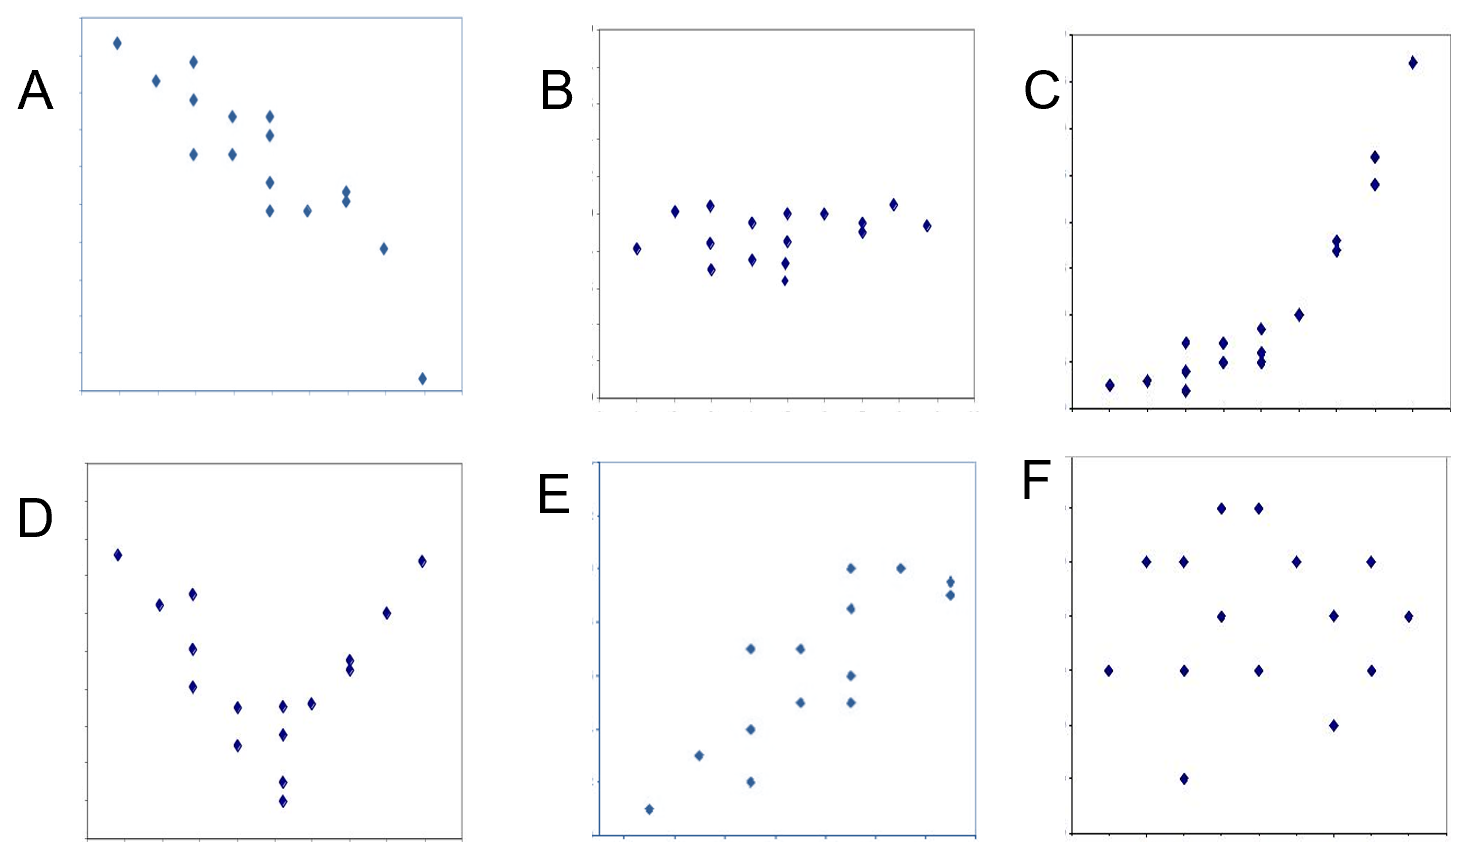
\includegraphics[scale=0.8]{images/scatters2.png}
\end{center}

\newpage

Caution:

\begin{center}
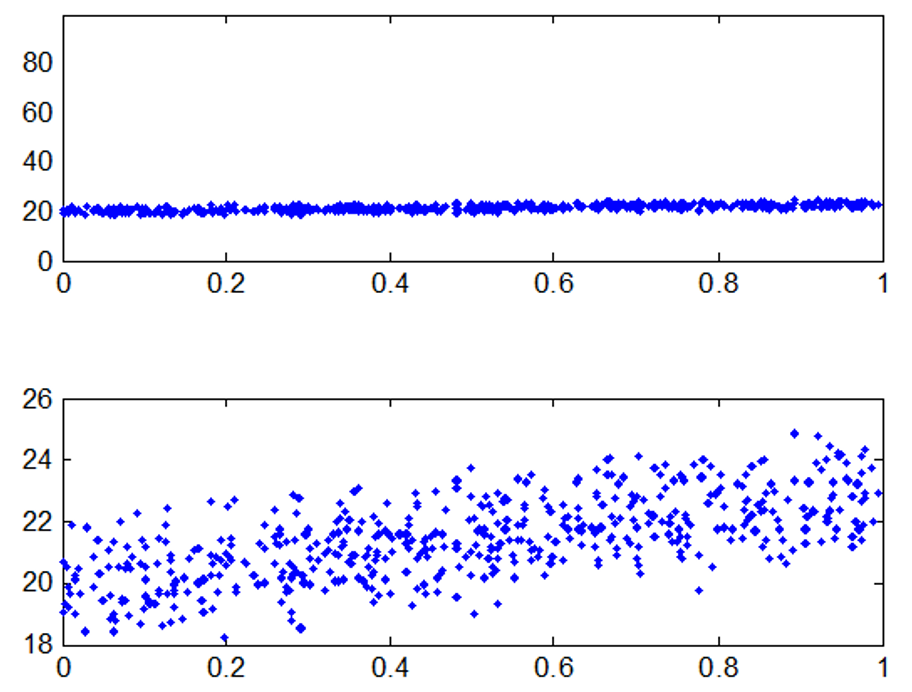
\includegraphics[scale=1]{images/scatters3.png}
\end{center}

\label{totalpag}
\end{document}